%==================================================================
%   Studienprojekt 2 -- Bericht (Kurzfassung, max. 20 Seiten)
%   TinyML-Sturzerkennung in der Einlegesohle
%   Aly Elbermawy · TH Mittelhessen · 2026
%
%   pdflatex main · bibtex main · pdflatex main · pdflatex main
%   Bilder in Bilder/: thm_logo.png, foto_platine*.jpg, *.tex (TikZ)
%==================================================================
\documentclass[11pt,a4paper,oneside,parskip=half,open=any,
               numbers=noenddot,listof=totoc,bibliography=totoc]{scrreprt}

\usepackage[utf8]{inputenc}
\usepackage[T1]{fontenc}
\IfFileExists{lmodern.sty}{\usepackage{lmodern}}{}
\usepackage[ngerman]{babel}
\usepackage[a4paper,left=2.5cm,right=2.3cm,top=2.3cm,bottom=2.4cm]{geometry}
\usepackage{microtype}
\usepackage{amsmath,amssymb}
\usepackage{graphicx}
\usepackage{xcolor}
\usepackage{booktabs,tabularx,array,multirow}
\usepackage{float}
\usepackage[font=small,labelfont=bf]{caption}
\usepackage{tikz}
\usetikzlibrary{arrows.meta,positioning,shapes.geometric,calc}
\usepackage[numbers,square,sort&compress]{natbib}
\bibliographystyle{ieeetr}
\usepackage[hidelinks]{hyperref}

\definecolor{thmgruen}{HTML}{80BA24}
\definecolor{thmgrau}{HTML}{4A5C66}
\definecolor{thmrot}{HTML}{B3263E}
\definecolor{thmblau}{HTML}{2F6DB5}

% Platzhalter fuer Ergebnisse, die erst nach dem naechsten Lauf vorliegen
\newcommand{\offen}[1]{\textcolor{red}{\textbf{[offen: #1]}}}
\newcommand{\ja}{\textcolor{thmgruen!70!black}{\textbf{bestätigt}}}
\newcommand{\nein}{\textcolor{thmrot}{\textbf{widerlegt}}}
\newcommand{\teils}{\textcolor{thmgrau}{\textbf{teilweise}}}
\newcolumntype{Y}{>{\raggedright\arraybackslash}X}
\newcolumntype{C}[1]{>{\centering\arraybackslash}p{#1}}

% Foto oder Rahmen mit Hinweis, falls die Datei noch fehlt
\newcommand{\foto}[3]{% Datei, Breite, Hinweistext
  \IfFileExists{Bilder/#1}{\includegraphics[width=#2]{Bilder/#1}}%
  {\fbox{\parbox[c][0.6#2][c]{\dimexpr#2-2\fboxsep-2\fboxrule\relax}{\centering\small\color{black!50}#3}}}}

\setkomafont{chapter}{\Large\bfseries}
\setkomafont{section}{\large\bfseries}
\RedeclareSectionCommand[beforeskip=-0.5\baselineskip,afterskip=0.8\baselineskip]{chapter}
\RedeclareSectionCommand[beforeskip=-0.8\baselineskip,afterskip=0.3\baselineskip]{section}
\RedeclareSectionCommand[beforeskip=-0.6\baselineskip,afterskip=0.2\baselineskip]{subsection}
\renewcommand{\chapterpagestyle}{plain}
\setlength{\floatsep}{8pt}\setlength{\textfloatsep}{10pt}\setlength{\intextsep}{8pt}

\begin{document}

%------------------------------------------------------------------
%   Titelseite
%------------------------------------------------------------------
\begin{titlepage}
\centering
\IfFileExists{Bilder/thm_logo.pdf}{\includegraphics[width=6.5cm]{Bilder/thm_logo.pdf}}{%
\IfFileExists{Bilder/thm_logo.png}{
\includegraphics[width=10cm]{Bilder/thm_logo.png}}{%
\IfFileExists{Bilder/thm_logo.jpg}{\includegraphics[width=6.5cm]{Bilder/thm_logo.jpg}}{%
{\Huge\bfseries\color{thmgrau} THM\par}\vspace{2pt}
{\small\color{thmgrau} TECHNISCHE HOCHSCHULE MITTELHESSEN\par}}}}
\par\vspace{0.4cm}
{\small Campus Friedberg\par}
\vspace{2.4cm}
{\large Studienprojekt 2 · Masterstudiengang Mechatronik\par}
\vspace{0.9cm}
{\color{thmgruen}\rule{0.8\textwidth}{1.2pt}}\\[0.5cm]
{\LARGE\bfseries Sturzerkennung mit TinyML\\[0.25cm] in einer sensorischen Einlegesohle\par}
\vspace{0.35cm}
{\large Vom Rumpf zum Fuß: Datensätze, Modelltransfer,\\Sensororientierung und Prototyp auf dem ESP32-C6\par}
{\color{thmgruen}\rule{0.8\textwidth}{1.2pt}}
\vfill
\begin{tabular}{@{}ll@{}}
\textbf{Verfasser:}       & Aly Elbermawy (Matr.-Nr.\ 5335848) \\
\textbf{Betreuer:}        & Prof.\ Dr.\ Sergej Kovalev \\
\textbf{Industriepartner:}& TrackTech GmbH / Clever-Sole, Friedberg \\
\textbf{Abgabe:}          & Oktober 2026 \\
\end{tabular}
\vspace{1.2cm}
\end{titlepage}

%------------------------------------------------------------------
%   Kurzfassung + Inhalt
%------------------------------------------------------------------
\pagenumbering{roman}
\section*{Kurzfassung}
Ziel des Projekts ist eine Sturzerkennung, die vollständig in einer
Einlegesohle auf einem ESP32-C6 mit sechsachsiger \emph{Inertial
Measurement Unit} (IMU) läuft. Öffentliche Sturzdatensätze messen fast
ausschließlich am Rumpf; einen Datensatz mit Stürzen an der Sohle gibt es
nicht. Ein 1D-CNN (61\,601 Parameter, int8 rund $77$\,KB) erreicht auf
SisFall $99{,}0\,\%$ Sensitivität bei $99{,}3\,\%$ Spezifität, verliert
aber an Bein und Fuß den Großteil seiner Leistung. Schrittweise wird
gezeigt, woran das liegt und was hilft: Sturzdaten vom Schienbein heben
die Sensitivität am Bein von $21$ auf $83\,\%$, treiben aber die
Fehlalarme an der Sohle auf mehrere hundert je Stunde; Sohlendaten ohne
Stürze senken sie um $91$--$96\,\%$, ohne Sensitivität zu kosten. Als bislang unbeachtete Fehlerquelle erweist sich die
\textbf{Achsenlage des Sensors}: Spiegelbildlich getragene Sensoren
unterscheiden sich bei identischen Stürzen um bis zu Faktor neun, und
allein die Ausrichtung der eigenen Hüftaufnahmen an den Achsen von
SisFall hebt die Erkennung von $2$ auf $15$ von $22$ Stürzen.
Eine Rotationsaugmentierung macht das Modell signifikant robuster. Auf
dem eigenen Prototyp erkennt das Modell nach Ausrichtung über die
Schwerkraft -- wie in der Firmware -- alle $67$ Stürze einer Person an
Hüfte und Knöcheln. Alle Aussagen sind subjektunabhängig
kreuzvalidiert und, wo möglich, gepaart statistisch abgesichert.

\vspace{0.3cm}
{\small\setcounter{tocdepth}{1}\tableofcontents}
\clearpage
\pagenumbering{arabic}

%==================================================================
\chapter{Theoretischer Hintergrund}
\label{ch:theorie}
%==================================================================

\section{Motivation und Aufgabenstellung}
Stürze sind bei älteren und pflegebedürftigen Menschen eine der
häufigsten Ursachen schwerer Verletzungen; entscheidend ist oft nicht
der Sturz selbst, sondern wie lange die Person unbemerkt liegen bleibt.
Der Projektpartner Clever-Sole entwickelt eine sensorische Einlegesohle.
Das Studienprojekt untersucht, ob sich darin eine Sturzerkennung
\emph{auf dem Gerät} (TinyML) realisieren lässt. Die Aufgaben umfassen
(1) die Wahl der Sensorkonfiguration, (2) die relevanten
Sensoreigenschaften, (3) die Bewertung öffentlicher Datensätze und
(4) Entwicklung, Training und prototypische Integration des Modells.
Der Schwerpunkt liegt auf Aufgabe~4.

\section{Sensorik: Achsen und Sensoreigenschaften}
Ein \textbf{3-Achsen}-Beschleunigungssensor erfasst Aufprall und
Freifall über den Betrag $|a|$, kann aber sturzähnliche
Alltagsaktivitäten (\emph{Activities of Daily Living}, ADL) wie
kräftiges Hinsetzen schlecht abgrenzen \cite{dinh2021,huynh2015}. Ein
\textbf{Gyroskop} (6 Achsen) ergänzt die Drehrate, also die für einen
Sturz typische schnelle Rotation in die Horizontale; in der Literatur
steigt dadurch vor allem die Spezifität, z.\,B.\ von $82{,}7$ auf
$96{,}2\,\%$ \cite{huynh2015}. Ein \textbf{Magnetometer} (9 Achsen)
liefert eine absolute Richtung und korrigiert die Gyroskopdrift
\cite{roetenberg2005}. Diese Drift ist über die ein bis zwei Sekunden
eines Sturzes vernachlässigbar, während Magnetfelder in Innenräumen
durch Stahl und Geräte gestört werden \cite{pmc11991382}. Empfohlen
wird daher eine \textbf{6-Achsen-IMU}; Tabelle~\ref{tab:eigenschaften}
fasst den Arbeitspunkt zusammen.

\begin{table}[H]
\centering\small
\caption{Sensoreigenschaften und empfohlener Arbeitspunkt.}
\label{tab:eigenschaften}
\begin{tabularx}{\textwidth}{l Y l}
\toprule
\textbf{Eigenschaft} & \textbf{Wirkung auf die Sturzerkennung} & \textbf{Empfehlung} \\
\midrule
Messbereich   & Zu klein: Aufprallspitze wird abgeschnitten (Clipping) \cite{cornelissen2023clipping} & $\pm 16$\,g \\
Abtastrate    & $15$--$20$\,Hz genügen dem CNN \cite{villar2022sampling,diaz2026sampling}; Erfassung höher, dann filtern & $\geq 100$\,Hz $\rightarrow$ $50$\,Hz \\
Auflösung     & Effektiv durch Rauschen begrenzt \cite{nxp2013an4075} & $\geq 12$\,Bit \\
Rauschdichte  & Relevant für feine Merkmale, nicht für den Aufprall \cite{arar2022noise} & $\lesssim 100\,\mu$g$/\sqrt{\text{Hz}}$ \\
Gyroskopdrift & Über die Sturzdauer vernachlässigbar \cite{roetenberg2005} & unkritisch \\
\bottomrule
\end{tabularx}
\end{table}

\section{Verfahren der Sturzerkennung}
\textbf{Schwellwertverfahren} lösen aus, wenn $|a|$ einen Freifall- und
einen Aufprallschwellwert über- bzw.\ unterschreitet \cite{bagala2012}.
\textbf{Klassische ML-Verfahren} wie der Random Forest arbeiten auf
Merkmalen je Zeitfenster; beruhen diese auf Vektorbeträgen, sind sie
unabhängig von der Einbaulage. Ein \textbf{1D-CNN} lernt die Merkmale
direkt aus dem Rohsignal (Fenster $T \times 6$). Es ist dadurch
leistungsfähiger, verarbeitet die sechs Kanäle aber einzeln und ist
\emph{nicht} drehinvariant: Dieselbe Bewegung erscheint bei gedrehtem
Sensor in anderen Kanälen.

\textbf{Domänenlücke und Transfer Learning.} Ein Modell, das an einer
Position und mit einer Sensorhardware trainiert wurde, überträgt sich
nicht zwangsläufig auf eine andere (\emph{Domänenlücke}). Beim
Fine-Tuning werden die Gewichte eines vortrainierten Modells mit
kleiner Lernrate auf Daten der Zieldomäne nachtrainiert, bei
progressivem Fine-Tuning über eine Zwischendomäne.

\textbf{Orientierung.} Wird der Sensor um eine Rotationsmatrix $R$
gedreht, gilt für Beschleunigung und Drehrate $a' = R\,a$,
$\omega' = R\,\omega$. Bei einer Spiegelung (linke statt rechte Körperseite)
verhält sich $\omega$ als Pseudovektor: Die gespiegelte Achse der
Beschleunigung wechselt das Vorzeichen, beim Gyroskop die beiden anderen.
Eine \textbf{Rotationsaugmentierung} ergänzt das Training um zufällig
gedrehte und gespiegelte Kopien jedes Fensters, damit das CNN die
Orientierung nicht als Merkmal lernt.

\textbf{Bewertungsgrößen.} Sensitivität $Se = TP/(TP+FN)$ (erkannte
Stürze), Spezifität $Sp = TN/(TN+FP)$, Genauigkeit $Acc$ und -- für den
Einsatz entscheidend -- \textbf{Fehlalarme je Stunde} Alltag (FP/h).
Bei seltenen Stürzen ist die Genauigkeit wenig aussagekräftig: Ein
Modell, das nie alarmiert, erreicht bereits über $97\,\%$.

\section{Datensätze}
Tabelle~\ref{tab:daten} und Abbildung~\ref{fig:koerper} zeigen die
verwendeten Datensätze und ihre Messorte. Kein Datensatz enthält
Stürze an der Sohle; die beiden Sohlendatensätze enthalten nur Alltag.
MobiAct wurde wegen Smartphone-Sensorik ($\pm 2$\,g) und
nicht-kommerzieller Lizenz nicht verwendet, UniMiB-SHAR
(nur Beschleunigung) nur für den Achsenvergleich.

\begin{table}[H]
\centering\footnotesize
\setlength{\tabcolsep}{3.5pt}
\caption{Verwendete Datensätze (P: Probanden, S: Stürze vorhanden).}
\label{tab:daten}
\begin{tabularx}{\textwidth}{l l c c c Y}
\toprule
\textbf{Datensatz} & \textbf{Position} & \textbf{Hz} & \textbf{P} & \textbf{S} & \textbf{Rolle im Projekt} \\
\midrule
SisFall \cite{sucerquia2017sisfall}   & Hüfte                 & 200 & 38 & ja   & Basismodell \\
KFall \cite{kfall2021}                & unterer Rücken        & 100 & 32 & ja   & Transfer, Zwischenstufe \\
UMAFall \cite{umafall2017}            & 5 Positionen          & 20  & 19 & ja   & Transfer, Knöchel \\
FallAllD \cite{fallalld2020}          & Nacken, Hand, Taille  & 238 & 15 & ja   & Transfer \\
WEDA-FALL \cite{wedafall2023}         & Handgelenk            & 50  & 25 & ja   & Ältere (77--95 J.) \\
CAPPIMU \cite{cappimu2024}            & 9 Positionen          & 50  & 30 & ja   & Positionskurve, Beinmodell \\
ImbalanSense \cite{imbalansense2026}  & Sohle                 & 100 & 40 & nein & Alltag am Fuß (Training) \\
Smart-Insole \cite{smartinsole2021}   & Sohle                 & 100 & 29 & nein & externer Test, Vorher/Nachher \\
Eigene Pilotdaten                     & Hüfte, Knöchel        & 100 & 1  & ja   & Test auf Zielhardware \\
\bottomrule
\end{tabularx}
\end{table}

\begin{figure}[H]
\centering
\resizebox{0.86\textwidth}{!}{% Sensorpositionen der verwendeten Datensaetze (wird per \input eingebunden)
\begin{tikzpicture}[x=1cm,y=1cm,
  koerper/.style={fill=black!12,draw=black!35,line width=0.4pt},
  glied/.style={line width=11pt,line cap=round,draw=black!12},
  sturz/.style={circle,fill=thmrot,draw=white,line width=0.6pt,inner sep=2.2pt},
  adl/.style={rectangle,fill=thmblau,draw=white,line width=0.6pt,inner sep=2.2pt},
  pilot/.style={star,star points=5,fill=black!80,draw=white,line width=0.4pt,inner sep=1.5pt},
  ziel/.style={circle,draw=thmgruen,line width=1.6pt,inner sep=4pt},
  lab/.style={font=\scriptsize,align=left,inner sep=1pt},
  labr/.style={font=\scriptsize,align=right,inner sep=1pt},
  zeiger/.style={draw=black!45,line width=0.35pt}]

% --- Silhouette ---------------------------------------------------
\draw[glied] (-0.95,6.15) -- (-1.35,4.85) -- (-1.55,3.65);   % Arm rechts (Bildlinks)
\draw[glied] ( 0.95,6.15) -- ( 1.35,4.85) -- ( 1.55,3.65);   % Arm links
\draw[glied] (-0.42,3.9) -- (-0.47,2.0) -- (-0.5,0.55);       % Bein rechts
\draw[glied] ( 0.42,3.9) -- ( 0.47,2.0) -- ( 0.5,0.55);       % Bein links
\fill[black!12] (-0.62,0.22) ellipse (0.36 and 0.17);
\fill[black!12] ( 0.62,0.22) ellipse (0.36 and 0.17);
\draw[koerper,draw=none] (-1.05,6.35) .. controls (-1.1,5.2) and (-0.8,4.6) .. (-0.82,3.7)
  -- (0.82,3.7) .. controls (0.8,4.6) and (1.1,5.2) .. (1.05,6.35)
  .. controls (0.5,6.6) and (-0.5,6.6) .. cycle;               % Rumpf
\fill[black!12] (-0.16,6.45) rectangle (0.16,6.85);            % Hals
\fill[black!12] (0,7.25) circle (0.42);                        % Kopf

% --- Positionen ---------------------------------------------------
% Kopf
\node[sturz] (kopf) at (0.18,7.45) {};
\draw[zeiger] (kopf) -- (2.4,7.45) node[lab,right] {Kopf: CAPPIMU};
% Nacken
\node[sturz] (nacken) at (0,6.7) {};
\draw[zeiger] (nacken) -- (-2.4,7.0) node[labr,left] {Nacken: FallAllD};
% Brust
\node[sturz] (brust) at (0.3,5.75) {};
\draw[zeiger] (brust) -- (2.4,6.5) node[lab,right] {Brust: CAPPIMU, UMAFall};
% Oberarme
\node[sturz] (oar) at (-1.3,5.05) {};
\node[sturz] (oal) at ( 1.3,5.05) {};
\draw[zeiger] (oal) -- (2.4,5.6) node[lab,right] {Oberarm l./r.: CAPPIMU};
% Handgelenke
\node[sturz] (hgr) at (-1.53,3.85) {};
\node[sturz] (hgl) at ( 1.53,3.85) {};
\draw[zeiger] (hgl) -- (2.4,4.35) node[lab,right] {Handgelenk: CAPPIMU, UMAFall,\\FallAllD, WEDA-FALL};
% Huefte / Taille
\node[sturz] (huefte) at (0,4.05) {};
\node[pilot] (hpilot) at (0.32,4.05) {};
\draw[zeiger] (huefte) -- (-2.4,4.95) node[labr,left] {Hüfte/Taille: \textbf{SisFall},\\UMAFall, FallAllD,\\eigener Prototyp};
\draw[zeiger] (-0.3,4.3) -- (-2.4,6.25) node[labr,left] {unterer Rücken: KFall};
\node[sturz] (ruecken) at (-0.3,4.3) {};
% Hosentasche
\node[sturz] (tasche) at (-0.62,3.35) {};
\draw[zeiger] (tasche) -- (-2.4,3.4) node[labr,left] {Hosentasche: CAPPIMU,\\UMAFall};
% Schienbein
\node[sturz] (sbr) at (-0.47,1.75) {};
\node[sturz] (sbl) at ( 0.47,1.75) {};
\draw[zeiger] (sbl) -- (2.4,2.6) node[lab,right] {oberes Schienbein l./r.:\\CAPPIMU};
% Knoechel
\node[sturz] (knr) at (-0.5,0.62) {};
\node[pilot] (knpr) at (-0.82,0.75) {};
\node[pilot] (knpl) at ( 0.82,0.75) {};
\draw[zeiger] (knr) -- (-2.4,1.25) node[labr,left] {Knöchel: UMAFall,\\eigener Prototyp (l./r.)};
% Sohle
\node[adl] (sohle) at (0.62,0.22) {};
\node[ziel] at (0.62,0.22) {};
\draw[zeiger] (sohle) -- (2.4,0.3) node[lab,right] {Sohle: ImbalanSense,\\Smart-Insole; \textbf{Zielposition}};

% --- Legende ------------------------------------------------------
\begin{scope}[shift={(-4.9,-0.75)}]
  \node[sturz] at (0,0) {}; \node[lab,right] at (0.15,0) {mit Stürzen};
  \node[adl] at (2.2,0) {};  \node[lab,right] at (2.35,0) {nur Alltag};
  \node[pilot] at (4.2,0) {}; \node[lab,right] at (4.35,0) {Pilotaufnahmen};
  \node[ziel] at (6.85,0) {}; \node[lab,right] at (7.1,0) {Zielposition};
\end{scope}
\end{tikzpicture}
}
\caption{Messorte der Datensätze am Körper. Stürze liegen nur an Rumpf,
Armen, Schienbein und Knöchel vor; an der Sohle nur Alltagsdaten.}
\label{fig:koerper}
\end{figure}

%==================================================================
\chapter{Durchführung}
\label{ch:durchfuehrung}
%==================================================================

\section{Prototyp und Datenaufnahme}
Der Prototyp besteht aus einem Seeed Studio XIAO ESP32-C6 (RISC-V,
$160$\,MHz, BLE, USB-C) und einem IMU-Modul (HW-123, Aufdruck MPU-6050;
die Firmware erkennt den Chip über das Register \texttt{WHO\_AM\_I}), verbunden
über I\textsuperscript{2}C und versorgt über einen Akkuanschluss
(Abbildung~\ref{fig:fotos}). Die IMU läuft mit $\pm 16$\,g,
$\pm 2000\,^{\circ}$/s und $100$\,Hz bei aktivem digitalem Tiefpassfilter.
Für die Pilotdaten wurde eine eigene Firmware (\emph{DatenLogger})
geschrieben: Aufnahme mit $100$\,Hz in den internen Flash, Bedienung per
Smartphone über Bluetooth (Aktivität wählen, Start/Stopp), automatischer
Stopp nach $120$\,s und Auslesen per Python-Skript. Da
Flash-Schreibzugriffe einzelne Abtastwerte verzögern, werden die Daten
anhand der Zeitstempel auf ein exaktes $100$-Hz-Raster interpoliert.

\begin{figure}[H]
\centering
\begin{minipage}[b]{0.25\textwidth}\centering
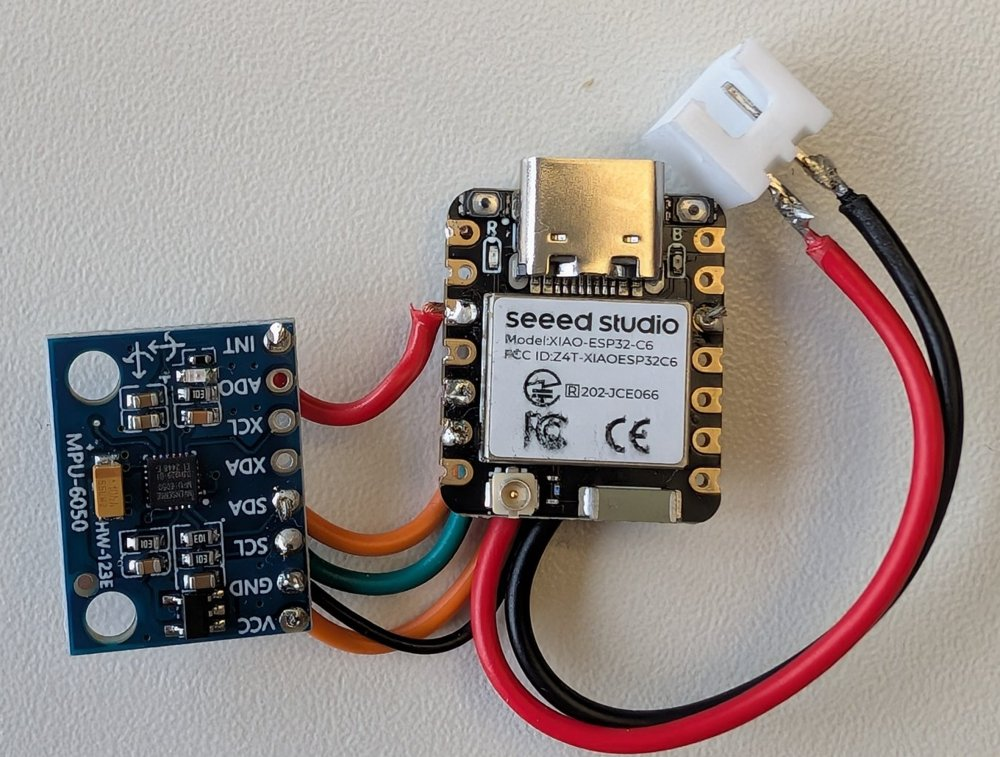
\includegraphics[width=\linewidth]{Bilder/foto_platine.jpg}\\[1pt]
{\footnotesize (a) Oberseite}
\end{minipage}\hspace{2mm}%
\begin{minipage}[b]{0.25\textwidth}\centering
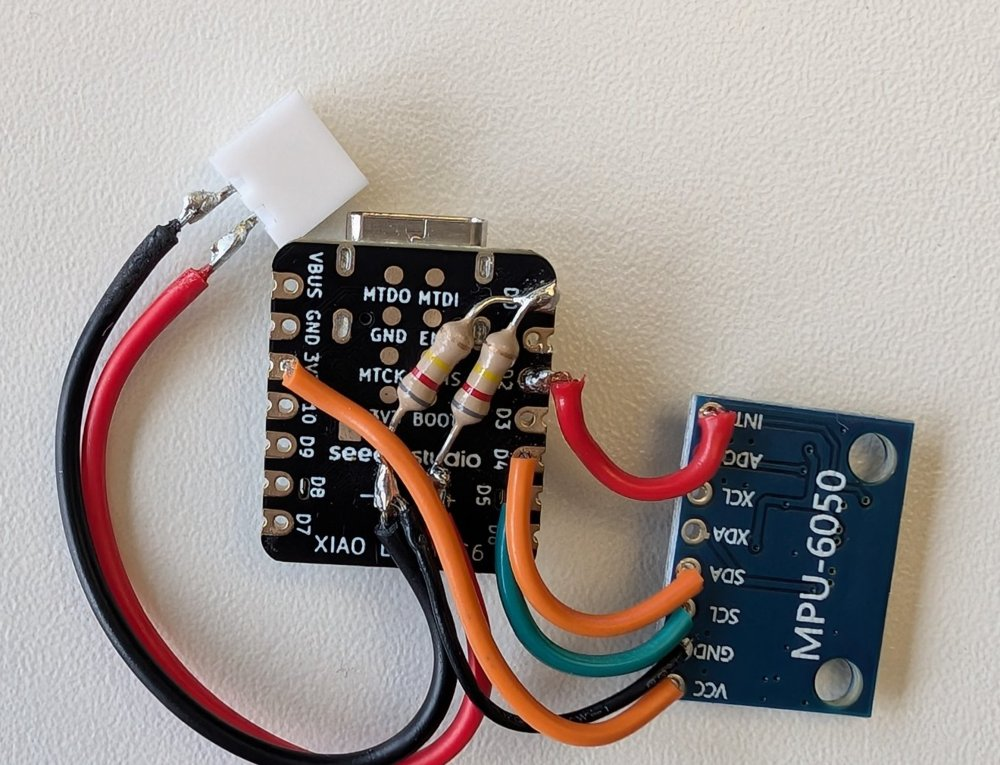
\includegraphics[width=\linewidth]{Bilder/foto_platine_unten.jpg}\\[1pt]
{\footnotesize (b) Unterseite}
\end{minipage}\hspace{2mm}%
\begin{minipage}[b]{0.44\textwidth}\centering
\resizebox{\linewidth}{!}{% Einbaulage des Prototyps: (a) Knoechel, Seitenansicht; (b) Sohle, Draufsicht
\begin{tikzpicture}[x=1cm,y=1cm,
  bein/.style={fill=black!10,draw=black!40,line width=0.5pt},
  platine/.style={fill=thmgrau!85,draw=black!70,line width=0.4pt,rounded corners=0.5pt},
  usb/.style={fill=black!25,draw=black!70,line width=0.3pt},
  pf/.style={-{Stealth[length=2mm]},line width=0.8pt},
  txt/.style={font=\scriptsize,align=center}]

% ---------------- (a) Knoechel, Seitenansicht von aussen ----------------
\begin{scope}
  % Unterschenkel und Fuss (Blick auf die Aussenseite, Zehen rechts)
  \draw[bein] (-0.55,4.2) -- (-0.5,1.3) .. controls (-0.55,0.75) and (-0.75,0.5) .. (-0.75,0.25)
    .. controls (-0.75,0.0) and (-0.6,-0.05) .. (-0.3,-0.05) -- (2.3,-0.05)
    .. controls (2.6,-0.05) and (2.65,0.25) .. (2.35,0.35)
    .. controls (1.6,0.55) and (0.9,0.8) .. (0.55,1.3) -- (0.55,4.2);
  \draw[black!30] (-0.05,0.55) circle (0.13);                      % Knoechel
  % Platine an der Aussenseite oberhalb des Knoechels, USB-C oben
  \draw[platine] (-0.28,0.95) rectangle (0.18,1.55);
  \draw[usb] (-0.14,1.55) rectangle (0.04,1.68);
  \draw[pf,thmrot] (-0.05,1.75) -- (-0.05,2.45) node[above,txt,text=thmrot] {USB-C\\oben};
  \draw[pf,thmgruen!70!black] (0.25,1.25) -- (1.05,1.25) node[right,txt,text=thmgruen!70!black] {vorn};
  \node[txt] at (0.9,-0.5) {Knöchel, Seitenansicht};
  \node[txt,text=black!60] at (0.9,-0.85) {Bauteilseite außen};
\end{scope}

% ---------------- (b) Sohle, Draufsicht (rechter Fuss) ----------------
\begin{scope}[shift={(5.6,0)}]
  % Sohlenumriss, Ferse unten, Zehen oben; Aussenseite rechts
  \draw[bein] (0,0) .. controls (-0.75,0) and (-0.8,0.9) .. (-0.65,1.7)
    .. controls (-0.55,2.4) and (-0.95,3.2) .. (-0.6,3.9)
    .. controls (-0.3,4.45) and (0.55,4.45) .. (0.8,3.8)
    .. controls (1.0,3.2) and (0.75,2.4) .. (0.75,1.7)
    .. controls (0.75,0.9) and (0.75,0) .. (0,0);
  % IMU-Modul flach unter der Ferse, Chip oben, X-Pfeil zu den Zehen

  \fill[thmblau] (-0.25,0.45) rectangle (0.3,1.0);                 % IMU-Modul (blau)
  \draw[pf,white] (0.02,0.55) -- (0.02,0.92);                        % X-Pfeil zu den Zehen
  \draw[pf,thmrot] (0.42,0.95) -- (1.3,1.45) node[right,txt,text=thmrot] {X-Pfeil des\\IMU-Moduls\\zu den Zehen};
  \node[txt] at (0.05,2.3) {Sohle};
  \draw[pf,thmgruen!70!black] (-1.2,1.6) -- (-1.2,2.6) node[above,txt,text=thmgruen!70!black] {Zehen};
  \node[txt] at (0.1,-0.5) {Sohle, Draufsicht};
  \node[txt,text=black!60] at (0.1,-0.85) {Chip oben, selbst kalibriert};
\end{scope}
\end{tikzpicture}
}\\[1pt]
{\footnotesize (c) Einbaulage: Pilotaufnahmen (Knöchel), Zielposition (Sohle)}
\end{minipage}
\caption{Prototyp: XIAO ESP32-C6 mit IMU-Modul und Akkuanschluss (a, b)
sowie Einbaulage des Sensors (c).}
\label{fig:fotos}
\end{figure}

\textbf{Aufnahmeprotokoll.} Eine Person (der Verfasser) trug den Sensor
an der Hüfte sowie am rechten und linken Knöchel (USB-Buchse jeweils
oben). Je Position wurden vier Sturzarten auf eine Matte aufgezeichnet
(auf die Knie, vorwärts, seitlich, rückwärts; je vier bis acht
Wiederholungen mit anschließender Liegephase von $5$\,s) sowie Gehen,
Joggen, Treppen, Hinsetzen, kräftiges Hinsetzen, Springen, Aufheben
und Hinlegen. Insgesamt liegen $22$/$23$/$22$ Stürze und
$9{,}7$/$6{,}6$/$7{,}2$\,min Alltag (Hüfte/Knöchel rechts/links) vor.
Aufnahmen in beiden Sohlen (vier Sturzarten, Alltag) entstanden erst
zum Projektende; sie werden in Abschnitt~\ref{sec:sohle} beschrieben,
aber noch nicht mit dem Modell ausgewertet.

\section{Datenaufbereitung}
Alle Datensätze werden in eine gemeinsame Form gebracht: sechs Kanäle in
g und $^{\circ}$/s, gefiltertes Heruntertasten auf $50$\,Hz, Fenster von
$2$\,s ($100 \times 6$) und Z-Normalisierung je Fenster und Kanal. Ein
Sturzfenster wird auf den Aufprall (Maximum von $|a|$) zentriert;
innerhalb einer Sturzaufnahme gilt \emph{nur} dieses Fenster als Sturz.
Zwei Sonderfälle erforderten eigene Lösungen:

\begin{itemize}\setlength\itemsep{1pt}
\item \textbf{CAPPIMU} beschriftet eine ganze Sturzsitzung ($\approx 160$\,s)
      als \emph{fall}. Einzelne Aufpralle werden an der Brust detektiert
      ($>2{,}5$\,g, Abstand $\geq 4$\,s) und über die gemeinsamen
      Zeitstempel auf alle Positionen übertragen.
\item \textbf{Pilotdaten:} Am Knöchel ist der Sturz ($2{,}6$--$2{,}9$\,g
      im Median) oft schwächer als Klopfmarken oder Springen (bis
      $12$\,g). Der Aufprall wird daher über die folgende Liegephase
      bestimmt: Ruhe $\geq 2$\,s, deren Schwerkraftrichtung um mehr als
      $40^{\circ}$ von der Stehhaltung abweicht; Aufprall ist das Maximum
      von $|a|$ in den $2$\,s davor.
\end{itemize}

\section{Modelle und Trainingskette}
Das CNN besteht aus drei Faltungsblöcken (32/64/128 Filter, Kernel 5,
Batch-Normalisierung, Max-Pooling), Global-Average-Pooling, einer
Dense-Schicht (64) mit Dropout $0{,}3$ und Sigmoid-Ausgang (61\,601
Parameter, Adam, binäre Kreuzentropie, Klassengewichte). Als
Vergleich dienen ein Schwellwertverfahren und ein Random Forest mit 18
Betragsmerkmalen. Abbildung~\ref{fig:kette} zeigt die Trainingskette
für das Fußmodell.

\begin{figure}[H]
\centering
\begin{tikzpicture}[node distance=4mm,
  box/.style={draw=thmgrau,rounded corners=2pt,align=center,font=\scriptsize,
              minimum height=10mm,text width=20mm,fill=white},
  pf/.style={-{Stealth[length=2mm]},thmgrau,line width=0.7pt}]
\node[box] (s) {\textbf{W}\\SisFall\\(Hüfte)};
\node[box,right=of s] (k) {\textbf{WK}\\+ KFall\\(Rücken)};
\node[box,right=of k,text width=27mm] (b) {\textbf{B1}\\+ CAPPIMU\\Schienbein (Stürze)};
\node[box,right=of b,text width=27mm,fill=thmgruen!12] (b2) {\textbf{B2 / B2r}\\+ ImbalanSense Sohle\\(Alltag) [+ Augm.]};
\node[box,right=of b2,text width=17mm,fill=black!6] (fw) {int8\\Firmware};
\draw[pf] (s)--(k); \draw[pf] (k)--(b); \draw[pf] (b)--(b2); \draw[pf] (b2)--(fw);
\end{tikzpicture}
\caption{Trainingskette vom Rumpf- zum Fußmodell. B2r: B2 mit
Rotations-/Spiegelaugmentierung (eine zufällig gedrehte, mit $50\,\%$
gespiegelte Kopie je Fenster).}
\label{fig:kette}
\end{figure}

\section{Bewertungsmethodik}
\begin{itemize}\setlength\itemsep{1pt}
\item \textbf{Subjektunabhängig:} Kein Proband erscheint zugleich in
      Training und Test.
\item \textbf{Fünffache Kreuzvalidierung, gepaart:} Verfahren werden auf
      denselben Falten verglichen; berichtet wird die mittlere Differenz
      mit $95\,\%$-Konfidenzintervall. Ein Unterschied gilt als
      gesichert, wenn das Intervall die Null nicht enthält.
      Konfidenzintervalle einzelner Anteile nach Wilson.
\item \textbf{Fehlalarme} auf reinen Alltagsdaten, umgerechnet je Stunde
      (Fenster mit $1$\,s Versatz, ohne Abstimmungsregel).
\item \textbf{Betriebsbewertung} wie in der Firmware: Inferenz alle
      $0{,}2$\,s, Alarm bei 3 von 5 Fenstern über $0{,}5$. Ein Sturz gilt
      als erkannt, wenn spätestens $1$\,s nach dem Aufprall ein Alarm
      fällt; jeder Alarm im Alltag ist ein Fehlalarm-Ereignis.
\end{itemize}
Der Code liegt in einer gemeinsamen Bibliothek (\texttt{fall\_lib.py})
und fünf Colab-Notebooks: (01) Basismodell, (02) Transfer, Fehlalarme,
Zielgruppe, (03) progressives Training, (04) Fuß und Orientierung,
(05) Pilotdaten und kommerzielles Modell.

\section{Firmware}
Die Firmware ist für die Einlegesohle ausgelegt. Sie liest die IMU mit
$100$\,Hz, tastet auf $50$\,Hz herunter, hält einen Ringpuffer von $2$\,s
und führt alle $200$\,ms eine Inferenz mit TensorFlow Lite Micro aus
(int8, $77$\,KB, 7 Operatoren). Eine 3-von-5-Regel entscheidet über den
Alarm, der per BLE gemeldet wird. Eingesetzt wird B2r, da es gegenüber
Drehungen am robustesten ist (Abschnitt~\ref{sec:orient}); int8 und
Gleitkommamodell treffen auf den Pilotfenstern in $99{,}5\,\%$ der Fälle
dieselbe Entscheidung.

\textbf{Batch-Normalisierung und Selbsttest.} Auf dem ESP32-C6 lieferte
das Modell zunächst unabhängig vom Eingang konstant $p \approx 0{,}47$,
während dieselbe Datei am PC korrekt rechnete. Ursache waren die aus der
Batch-Normalisierung entstehenden MUL/ADD-Operationen mit Broadcast, die
TFLite Micro dort falsch auswertet. Das Exportskript rechnet die
Normalisierung deshalb in die jeweils folgende Faltungs- bzw.
Dense-Schicht ein (maximale Abweichung $< 10^{-5}$) und legt fünf
Selbsttest-Muster samt Sollausgabe ab, die die Firmware beim Start
nachrechnet.

\textbf{Selbstkalibrierung der Einbaulage.} Vorgabe ist: IMU-Modul flach
unter der Ferse, Chip oben, aufgedruckter X-Pfeil zu den Zehen. Da die
Lage in einer Sohle nie exakt ist, bestimmt die Firmware sie nach jedem
Aufwachen selbst: Die Schwerkraft im Stillstand liefert die Hochachse,
die Hauptdrehachse der Winkelgeschwindigkeit beim Gehen die Querachse,
und die Schiefe der Drehrate um diese Achse (die Schwungphase erzeugt die
größten Spitzen) legt fest, wo vorn ist. Daraus folgt die Drehung in den
Trainingsrahmen ($x'$ vorwärts, $y'$ abwärts, $z'$ links). Auf den
Knöchelaufnahmen, rechnerisch in beliebige Lagen gedreht, stellte das
Verfahren die Achsen in allen Fällen richtig wieder her
(Vorwärtsstürze danach $x' = -0{,}89$ bis $-1{,}0$); an der Sohle ist es
noch zu bestätigen.

\textbf{Sturzrichtung und Testmodus.} Nach einem Alarm wertet die
Firmware die erste Ruhephase aus und meldet die Lage als Schätzung
(Bauchlage $\approx$ vorwärts, Rückenlage $\approx$ rückwärts, seitlich).
Das Modell selbst unterscheidet nur Sturz und Nicht-Sturz; seine Ausgabe
$p$ ist kein kalibrierter Wahrscheinlichkeitswert. Ein Testmodus sendet
jede Modellausgabe über BLE, um Versuche auszuwerten.

\section{Kommerzielles Modell}
Für den Projektpartner wird ein zweites Modell nur aus Daten trainiert,
deren Lizenz eine kommerzielle Nutzung nicht ausschließt:
\textbf{alle Datensätze außer Smart-Insole und MobiAct}. Es wird von
Grund auf auf einem gemischten Pool aller Positionen vortrainiert
(SisFall, KFall, UMAFall, FallAllD, WEDA-FALL, CAPPIMU ohne Schienbein;
orientierungsaugmentiert), dann wie B2r auf Schienbein und ImbalanSense
nachtrainiert und abschließend um die eigenen Pilotaufnahmen ergänzt.
Der Unterschied zum Berichtsmodell B2r prüft die Behauptung, dass
breiteres Vortraining dem Fußmodell nützt (Abschnitt~\ref{sec:kommerz}).
Die Lizenzen sind vor der Übergabe im Einzelnen zu prüfen.

%==================================================================
\chapter{Ergebnisse und Diskussion}
\label{ch:ergebnisse}
%==================================================================
Die Ergebnisse sind entlang der Behauptungen geordnet, die im Projekt
geprüft wurden. Tabelle~\ref{tab:hypothesen} am Ende des Kapitels fasst
zusammen, welche sich bestätigt haben und welche nicht.

\section{Basismodell am Rumpf}
\begin{table}[H]
\centering\small
\caption{Basismodelle auf SisFall, subjektunabhängiger Testsatz
(10 Probanden, 12\,431 Fenster). Quelle: Notebook~01.}
\label{tab:basis}
\begin{tabularx}{0.85\textwidth}{Y c c c r r}
\toprule
\textbf{Modell} & \textbf{Se} & \textbf{Sp} & \textbf{Acc} & \textbf{FP} & \textbf{FN} \\
\midrule
Schwellwert ($|a| > 2{,}8$\,g) & $96{,}7\,\%$ & $82{,}9\,\%$ & $83{,}2\,\%$ & 2\,074 & 10 \\
Random Forest (18 Betragsmerkmale) & $92{,}7\,\%$ & $99{,}6\,\%$ & $99{,}4\,\%$ & 48 & 22 \\
\textbf{1D-CNN} & $\mathbf{99{,}0\,\%}$ & $\mathbf{99{,}3\,\%}$ & $\mathbf{99{,}3\,\%}$ & 82 & \textbf{3} \\
\bottomrule
\end{tabularx}
\end{table}

Jede Stufe behebt die Schwäche der vorigen: Der Random Forest senkt die
Fehlalarm-Fenster des Schwellwerts um den Faktor $43$, das CNN die
übersehenen Stürze von 22 auf 3. Ein Schwellwert kann nur Sensitivität
gegen Fehlalarme tauschen: Bei $1{,}5$\,g erkennt er alle Stürze bei
$57{,}5\,\%$ Spezifität, bei $4{,}0$\,g noch $74{,}7\,\%$ der Stürze bei
$95{,}9\,\%$ Spezifität. Im Random Forest entfallen $62{,}3\,\%$ der
Merkmalswichtigkeit auf das Gyroskop. Der direkte Achsenvergleich mit
identischem CNN relativiert den Nutzen jedoch: mit 6 Achsen
$99{,}3\,\%$, nur mit Beschleunigung $98{,}0\,\%$, nur mit Gyroskop
$94{,}7\,\%$ Sensitivität. An der Hüfte liegt die Leistung nahe der
Obergrenze; der Vorteil des Gyroskops ($+1{,}3$\,pp) ist dort klein. Ein
mit 3 Achsen trainiertes Modell erreicht auf UniMiB-SHAR ($\pm 2$\,g,
Hosentasche) nach Fine-Tuning $95{,}5\,\%$ (Zero-Shot $23{,}5\,\%$).

\section{Übertragbarkeit auf andere Datensätze}
\begin{table}[H]
\centering\small
\caption{Transfer des SisFall-Modells. Zero-Shot (ZS) und nach
Fine-Tuning (FT), je eine subjektunabhängige Aufteilung. Quelle: Notebook~02.}
\label{tab:transfer}
\begin{tabularx}{\textwidth}{l l c c Y}
\toprule
\textbf{Datensatz} & \textbf{Position, Hz} & \textbf{Se ZS} & \textbf{Se FT} & \textbf{Anmerkung} \\
\midrule
KFall    & Rücken, 100   & $99{,}5\,\%$  & $100{,}0\,\%$ & Sp $99{,}5\,\%$ ohne Anpassung \\
UMAFall  & Taille, 20    & $45{,}8\,\%$  & $93{,}8\,\%$  & \\
UMAFall  & Knöchel, 20   & $25{,}0\,\%$  & $25{,}0\,\%$  & 36 Sturzfenster im Test; CV in Tab.~\ref{tab:prog} \\
FallAllD & Taille, 238   & $11{,}3\,\%$  & $75{,}8\,\%$  & Messbereich $\pm 8$\,g \\
\bottomrule
\end{tabularx}
\end{table}

KFall überträgt ohne Anpassung, FallAllD trotz der höchsten Abtastrate
kaum. Ein Kontrollversuch schließt den Messbereich als Ursache aus:
Auf $\pm 8$\,g und $\pm 4$\,g begrenzte SisFall-Testdaten erreichen
unverändert $99{,}0\,\%$, selbst $\pm 2$\,g noch $98{,}0\,\%$. Ursprünglich
wurde die Lücke den Signaleigenschaften der Hardware zugeschrieben. Die
Ergebnisse zur Orientierung (Abschnitt~\ref{sec:orient}) legen eine
einfachere Erklärung nahe: An der eigenen Hüfte bricht das Basismodell
ebenso ein und erholt sich allein durch Ausrichtung der Achsen. Für
FallAllD wurde dies nicht geprüft, ist aber naheliegend.

\section{Fehlalarme und zeitliche Plausibilisierung}
Auf den Alltagsdaten am Knöchel (UMAFall, $1{,}76$\,h) löst das
Basismodell $3{,}8\,\%$ der Fenster aus, rund $137$ Fehlalarme je Stunde,
vor allem beim Joggen ($20{,}1\,\%$), Türöffnen ($5{,}7\,\%$) und Gehen
($4{,}9\,\%$) -- also bei jedem Fersenaufsatz. Die Wahrscheinlichkeit liegt dabei bis $p = 1{,}000$;
eine höhere Schwelle allein hilft nicht.

Eine N-von-M-Regel verlangt $N$ positive unter den letzten $M$
Entscheidungen. Sie wirkt erst bei kleiner Schrittweite ($0{,}2$\,s):
Bei $1$\,s liegt der Aufprall in nur einem Fenster, sodass jede Regel mit
$N \geq 2$ scheitert. Auf UMAFall (47 Stürze, $0{,}57$\,h Alltag)
senkt \emph{3-von-5} die Fehlalarme des angepassten Modells um $70\,\%$
($246 \rightarrow 74$/h), kostet aber $40\,\%$ der erkannten Stürze
($25 \rightarrow 15$). Strengere Regeln lassen kaum Stürze übrig
(\emph{5-von-7}: 3 von 47 bei $40$/h). Das nicht angepasste Modell
erkennt mit 3-von-5 ebenso 15 Stürze, bei $98$/h. \textbf{Voting allein
löst das Fehlalarmproblem am Knöchel nicht}; es glättet nur, was das
Modell liefert.

\section{Progressives Training und Hard Negatives}
\begin{table}[H]
\centering\small
\caption{UMAFall-Knöchel, fünffach kreuzvalidiert (157 Stürze). Quelle: Notebook~03.}
\label{tab:prog}
\begin{tabularx}{\textwidth}{l Y c c}
\toprule
& \textbf{Strategie} & \textbf{Se [95\,\%-KI]} & \textbf{Sp} \\
\midrule
A  & Zero-Shot (SisFall)                          & $28{,}7\,\%$ [$22{,}2$; $36{,}2$] & $96{,}2\,\%$ \\
B  & direkt: SisFall $\rightarrow$ UMAFall          & $35{,}7\,\%$ [$28{,}6$; $43{,}4$] & $96{,}8\,\%$ \\
C1 & nur Zwischenstufe KFall                         & $12{,}7\,\%$ [$8{,}4$; $18{,}9$] & $98{,}6\,\%$ \\
C2 & progressiv: SisFall $\rightarrow$ KFall $\rightarrow$ UMAFall & $\mathbf{56{,}7\,\%}$ [$48{,}9$; $64{,}2$] & $96{,}8\,\%$ \\
\bottomrule
\end{tabularx}
\end{table}

Progressiv übertrifft direkt um $+23{,}8$\,pp (KI $[+3{,}9; +43{,}8]$,
3 von 5 Falten besser, 2 gleich; Spezifität unverändert), obwohl die
Zwischenstufe allein die Leistung zunächst
senkt (C1): Sie verallgemeinert die Repräsentation, statt sie zu
verbessern. Eine Höhergewichtung impactstarker Alltagsfenster
(\emph{Hard Negatives}, Faktor 3) hebt zwar die Spezifität um
$+1{,}8$\,pp, kostet aber $-6{,}3$\,pp Sensitivität (KI
$[-9{,}9; -2{,}6]$, beides gesichert, 5 von 5 Falten). Für ein Notrufsystem ist das der
falsche Tausch, denn Fehlalarme lassen sich nachgelagert filtern,
übersehene Stürze nicht.

Eine Einschränkung zeigt Abschnitt~\ref{sec:orient}: Mit vielen
Sturzdaten am Bein (CAPPIMU, 1462 Sturzfenster) ist ein Modell
\emph{ohne} Rumpf-Vortraining (L0) ebenso gut wie die progressive Kette
(B2; $+0{,}5$\,pp, nicht gesichert). Das Vortraining hilft also, wenn
Zieldaten knapp sind.

\section{Zielgruppe: ältere Menschen}
Auf WEDA-FALL (Handgelenk) erzeugen Ältere bei gleichen Aktivitäten
$4{,}0$-mal mehr Fehlalarme ($172$ gegenüber $43$/h, Schwelle $0{,}9$).
Die Aufschlüsselung zeigt, dass dies vor allem auf Klatschen
($21{,}0$ gegenüber $2{,}0\,\%$ der Fenster) und Türöffnen ($6{,}8$
gegenüber $0{,}8\,\%$) zurückgeht; beim Gehen ($0{,}2$ gegenüber
$0{,}4\,\%$) und Treppensteigen schneiden Ältere sogar besser ab. An der
Sohle (Smart-Insole) liegen Ältere ($127$/h) und Parkinson-Patienten
($120$/h) dagegen bei denselben Geh- und Aufstehtests deutlich über
jüngeren Erwachsenen ($69$/h). Für die Sohle
ist die Zielgruppe also ein realer Faktor.

\section{Vom Rumpf zum Fuß}
\textbf{Die Sohle ist die schwierigste Position.} Die Partnerdaten des
bestehenden Sohlenprototyps sind mit $10$\,Hz, $\pm 2$\,g je Achse
($6{,}4\,\%$ aller Achswerte am Anschlag, schon beim Gehen) und ohne
Gyroskop nicht verwendbar. Unverfälschte
Sohlendaten zeigen, warum: Schon beim Gehen erreicht $|a|$ im
99.~Perzentil $4{,}4$--$5{,}1$\,g, Einzelachsen bis $\pm 16$\,g -- mehr
als viele Stürze am Rumpf. Tabelle~\ref{tab:kurve} zeigt das unveränderte
Basismodell an allen Positionen.

\begin{table}[H]
\centering\small
\caption{Basismodell (Zero-Shot) je Position. CAPPIMU: dieselben Stürze
gleichzeitig an neun Positionen (je 731 Sturzfenster, $\approx 31$\,h Alltag).
Quelle: Notebook~04, Teil~A.}
\label{tab:kurve}
\begin{tabularx}{\textwidth}{Y c c | Y c c}
\toprule
\textbf{Position} & \textbf{Se} & \textbf{FP/h} & \textbf{Position} & \textbf{Se} & \textbf{FP/h} \\
\midrule
Kopf              & $28{,}5\,\%$ & 66  & Handgelenk rechts & $50{,}9\,\%$ & 133 \\
Brust             & $51{,}4\,\%$ & 81  & Hosentasche       & $21{,}2\,\%$ & 63 \\
Oberarm links     & $5{,}1\,\%$  & 45  & Schienbein links  & $12{,}2\,\%$ & 152 \\
Oberarm rechts    & $47{,}3\,\%$ & 72  & Schienbein rechts & $48{,}3\,\%$ & 43 \\
Handgelenk links  & $13{,}5\,\%$ & 83  & \textbf{Sohle} (ImbalanSense / Smart-Insole) & -- & \textbf{65 / 101} \\
\bottomrule
\end{tabularx}
\end{table}

Statt einer mit dem Abstand vom Rumpf fallenden Kurve unterscheiden sich
\textbf{linke und rechte Seite} bei identischen Stürzen um bis zu Faktor
neun -- ein Befund, dem Abschnitt~\ref{sec:orient} nachgeht. Zugleich
zeigt sich, warum ein Spitzenwert am Bein nicht trennen kann: Am
Schienbein liegt die Aufprallspitze eines Sturzes im Median bei
$2{,}9$--$3{,}0$\,g, das 99.~Perzentil des Alltags bei $9{,}9$--$10{,}2$\,g;
an der Brust ($5{,}0$ gegenüber $6{,}0$\,g) und am Kopf ($2{,}9$ gegenüber
$2{,}2$\,g) liegen beide noch nah beieinander.

\textbf{Vorher/Nachher: Daten vom Bein und vom Fuß.}
Tabelle~\ref{tab:fussdaten} zeigt, wie sich die Leistung mit jeder
Datenquelle ändert. Bewertet wird auf Testprobanden, die nicht im
Training waren; Smart-Insole ist außer in der letzten Zeile ein
vollständig externer Test. Die oberen vier Zeilen (ohne Augmentierung)
und die unteren drei (augmentiert) stammen aus zwei Läufen; verglichen
wird jeweils nur innerhalb eines Blocks.

\begin{table}[H]
\centering\small
\setlength{\tabcolsep}{4pt}
\caption{Wirkung von Bein- und Fußdaten, fünffach kreuzvalidiert
(1462 Sturzfenster am Schienbein). Quelle: Notebook~04, Teil~B (oben)
und Teil~E (unten).}
\label{tab:fussdaten}
\begin{tabularx}{\textwidth}{l Y c c c c}
\toprule
& & \multicolumn{2}{c}{\textbf{Schienbein}} & \multicolumn{2}{c}{\textbf{FP/h Sohle}} \\
\cmidrule(lr){3-4}\cmidrule(lr){5-6}
& \textbf{Training} & \textbf{Se [95\,\%-KI]} & \textbf{Sp} & \textbf{ImbalanSense} & \textbf{Smart-Insole} \\
\midrule
A  & SisFall (Basis)                              & $30{,}2\,\%$ [$27{,}9$; $32{,}6$] & $97{,}3\,\%$ & 65  & 101 \\
K  & + KFall                                     & $21{,}5\,\%$ [$19{,}5$; $23{,}7$] & $98{,}5\,\%$ & 105 & 115 \\
B1 & + Schienbein-Stürze (\emph{ohne} Fußdaten)   & $83{,}2\,\%$ [$81{,}2$; $85{,}0$] & $98{,}8\,\%$ & 268 & 400 \\
B2 & + ImbalanSense (Sohle, ohne Stürze)          & $77{,}6\,\%$ [$75{,}4$; $79{,}6$] & $90{,}3\,\%$ & 36  & 81 \\
\midrule
B1r & B1, augmentiert                            & $84{,}3\,\%$ [$82{,}4$; $86{,}1$] & $98{,}5\,\%$ & 350 & 310 \\
B2r & B1r + ImbalanSense, augmentiert            & $\mathbf{84{,}0\,\%}$ [$82{,}0$; $85{,}8$] & $96{,}0\,\%$ & $\mathbf{13{,}2}$ & $\mathbf{28{,}0}$ \\
& B2r + Smart-Insole im Training               & $82{,}1\,\%$ [$80{,}0$; $84{,}0$] & $98{,}1\,\%$ & $1{,}6$ & $11{,}1$ \\
\bottomrule
\end{tabularx}
\end{table}

Drei Befunde. (1) \textbf{Sturzdaten vom Bein sind entscheidend}:
$+61{,}5$\,pp Sensitivität (B1 gegenüber K, KI $[+59{,}3; +63{,}8]$,
5 von 5 Falten). (2) \textbf{Ohne Fußdaten explodieren die Fehlalarme an
der Sohle} ($268$ bis $400$/h): Das Modell lernt \glqq kräftiger
Beinimpuls = Sturz\grqq{}, und jeder Fersenaufsatz ist einer.
(3) \textbf{Fußdaten ohne Stürze beheben das -- ohne Sensitivitätsverlust
aber nur mit Augmentierung.} Augmentiert (B2r gegenüber B1r) sinken die
Fehlalarme um $96$ bzw.\ $91\,\%$ (Spezifität $+9{,}4$ bzw.\
$+8{,}1$\,pp, gesichert), die Sensitivität bleibt gleich ($-0{,}2$\,pp,
nicht verschieden). Ohne Augmentierung (B2 gegenüber B1) sinken die
Fehlalarme ebenfalls ($-87$ bzw.\ $-80\,\%$), dafür fällt die Spezifität
am Schienbein gesichert um $8{,}6$\,pp und die Sensitivität um
$5{,}8$\,pp (nicht gesichert). Im Gegensatz zu den Hard Negatives werden
hier keine vorhandenen Fenster umgewichtet, sondern Daten der
Zielposition ergänzt. Smart-Insole als zweite Sohlenquelle senkt die Fehlalarme zwar
weiter ($13{,}2 \rightarrow 1{,}6$ bzw.\ $28{,}0 \rightarrow 11{,}1$/h),
kostet aber gesichert Sensitivität ($-2{,}0$\,pp, KI $[-3{,}7; -0{,}2]$,
nur 1 von 5 Falten). Da die Lizenz zudem nicht-kommerziell ist, bleibt
B2r das eingesetzte Modell; die Zeile dient nur dem Bericht.
Die Genauigkeit wird nicht berichtet: Sie liegt bei seltenen Stürzen in
allen Zeilen über $90\,\%$, obwohl die Sensitivität zwischen $21$ und
$84\,\%$ schwankt.

\section{Einfluss der Sensororientierung}
\label{sec:orient}
\textbf{Spiegeltest.} Werden die Sensoren der linken Körperseite
rechnerisch an der $xz$-Ebene gespiegelt (Gyroskop als Pseudovektor),
erreicht das Basismodell dort die Werte der rechten Seite: Oberarm
$5{,}1 \rightarrow 53{,}8\,\%$, Handgelenk $13{,}5 \rightarrow 57{,}5\,\%$,
Schienbein $12{,}2 \rightarrow 48{,}3\,\%$. Umgekehrt fällt die gespiegelte
rechte Seite auf $4{,}4$, $7{,}7$ und $14{,}9\,\%$. \textbf{Der
Seitenunterschied ist damit vollständig durch die Achsenlage erklärt.}
Bei 20 zufälligen Drehungen schwankt die Sensitivität am Schienbein
zwischen $6$ und $58\,\%$.

\textbf{Gegenmaßnahme: Augmentierung.} Tabelle~\ref{tab:matrix}
vergleicht fünf Trainingsketten auf denselben Falten.

\begin{table}[H]
\centering\small
\caption{Trainingsketten, fünffach kreuzvalidiert. Gedreht: Mittel über
fünf zufällige Drehungen der Testdaten. Quelle: Notebook~04, Teil~D; alle fünf
Zeilen stammen aus demselben Lauf und denselben Falten, nur so ist der
Vergleich zwischen den Ketten zulässig.}
\label{tab:matrix}
\begin{tabularx}{\textwidth}{l Y c c c c}
\toprule
& & \multicolumn{2}{c}{\textbf{Se Schienbein}} & \multicolumn{2}{c}{\textbf{FP/h Sohle}} \\
\cmidrule(lr){3-4}\cmidrule(lr){5-6}
& \textbf{Kette} & \textbf{original} & \textbf{gedreht} & \textbf{IMB} & \textbf{SI} \\
\midrule
W   & SisFall                                 & $30{,}2\,\%$ & $27{,}1\,\%$ & 65  & 101 \\
WK  & SisFall $\rightarrow$ KFall              & $21{,}1\,\%$ & $16{,}8\,\%$ & 80  & 88 \\
L0  & Bein + Fuß \emph{ohne} Vortraining      & $83{,}6\,\%$ & $51{,}6\,\%$ & 4   & 18 \\
B2  & WK $\rightarrow$ Bein + Fuß             & $84{,}1\,\%$ & $57{,}9\,\%$ & 17  & 50 \\
B2r & wie B2, augmentiert                     & $\mathbf{84{,}7\,\%}$ & $\mathbf{75{,}8\,\%}$ & \textbf{5} & \textbf{16} \\
\bottomrule
\end{tabularx}
\end{table}

Die Augmentierung kostet nichts: gedreht $+17{,}9$\,pp (KI
$[+11{,}9; +23{,}9]$, 5 von 5 Falten), original $+0{,}8$\,pp (nicht
verschieden), Spezifität an Smart-Insole gesichert höher ($+1{,}0$\,pp),
an ImbalanSense nicht verschieden.

Die Fehlalarmraten dieser Tabelle sind nicht mit denen aus
Tabelle~\ref{tab:fussdaten} vergleichbar: beide Läufe verwenden
unterschiedliche Obergrenzen für die Alltagsstichprobe und
unterschiedliche Zufallsstartwerte, und die Fehlalarme an der Sohle
streuen zwischen den Falten erheblich (B1r: $65$ bis $755$/h). Für B2r
stehen deshalb hier $5$ bzw.\ $16$/h, in Tabelle~\ref{tab:fussdaten}
dagegen $13{,}2$ bzw.\ $28{,}0$/h. Belastbar ist jeweils nur der
Vergleich \emph{innerhalb} einer Tabelle.

\textbf{Eigene Hüfte in den SisFall-Rahmen.} SisFall definiert die Achsen
des Gürtelsensors als $+z$ vorwärts, $+y$ nach unten, $+x$ nach rechts
\cite{sucerquia2017sisfall}. Am Prototyp zeigte die Schwerkraft im Stand
auf $-x$, und die Liegelage nach Vorwärts- und Rückwärtsstürzen weist
$+z$ als Vorwärtsrichtung aus. Daraus folgt die feste Drehung
$x_S = -y$, $y_S = x$, $z_S = z$ samt Ausgleich der Platinenneigung
($\approx 25^{\circ}$) -- bestimmt aus der Einbaulage, nicht aus den
Ergebnissen. Das \emph{unveränderte} Basismodell erkennt danach
\textbf{15 statt 2 von 22 Stürzen} bei etwa gleicher Zahl an
Fehlalarmen (13 statt 12; Tabelle~\ref{tab:pilot}). Nur die
Achsenvertauschung ohne Ausgleich der Neigung bringt 8 von 22. Ebenso zeigte die Liegelage, dass der linke
Knöchelsensor gegenüber dem rechten um $180^{\circ}$ um die Hochachse
gedreht war.

\section{Pilotversuch auf der Zielhardware}
\begin{table}[H]
\centering\small
\caption{Betriebsbewertung auf den eigenen Aufnahmen (3 von 5, Schwelle
$0{,}5$): erkannte Stürze / Fehlalarm-Ereignisse. \glqq Lage über
Schwerkraft\grqq: Drehung der mittleren Schwerkraft im Stand auf die des
Trainings, wie in der Firmware. Quelle: Notebook~05. Alltag:
Hüfte $9{,}3$, rechts $6{,}2$, links $6{,}8$\,min mit gezielt
schwierigen Bewegungen (Springen, kräftiges Hinsetzen, Aufheben).}
\label{tab:pilot}
\begin{tabularx}{\textwidth}{Y c c c}
\toprule
\textbf{Modell} & \textbf{Hüfte} & \textbf{Knöchel rechts} & \textbf{Knöchel links} \\
\midrule
Basis (SisFall), Rohdaten          & 2/22 \,/\, 12  & 16/23 \,/\, 16 & 8/22 \,/\, 39 \\
Basis, Achsen wie SisFall          & 15/22 \,/\, 13 & -- & -- \\
Basis, Lage über Schwerkraft       & 13/22 \,/\, 6  & 14/23 \,/\, 9  & 15/22 \,/\, 7 \\
B2 (Bein + Fuß)                    & 11/22 \,/\, 93 & 17/23 \,/\, 28 & 10/22 \,/\, 35 \\
B2r (augmentiert)                  & 18/22 \,/\, 83 & 21/23 \,/\, 21 & 17/22 \,/\, 29 \\
B2r, Lage über Schwerkraft         & \textbf{22/22 \,/\, 65} & \textbf{23/23 \,/\, 12} & \textbf{22/22 \,/\, 17} \\
\bottomrule
\end{tabularx}
\end{table}

Ohne Lageausgleich erkennt B2r am Knöchel 17 bis 21 der Stürze und
liegt damit deutlich über B2. Richtet man die Aufnahmen wie die Firmware
über die Schwerkraft aus (Neigung $35$--$47^{\circ}$ am Knöchel), erkennt
B2r \textbf{alle 67 Stürze}, obwohl es weder diese Hardware noch diese
Person gesehen hat; am Knöchel bei $12$ bzw.\ $17$ Fehlalarm-Ereignissen.
Die Fehlalarme stammen aus Bewegungen, bei denen das Bein selbst in die
Horizontale kommt (Hinsetzen, Aufheben); an der Hüfte sind es mit $65$
in $9{,}3$\,min deutlich mehr -- sie ist aber nicht die Zielposition.
Eine Rate je Stunde ist aus wenigen Minuten solcher Aufnahmen nicht
ableitbar.

\textbf{Kennwerte je Aktivität.} Abbildung~\ref{fig:kennwerte} zeigt zwei
orientierungsunabhängige Kennwerte je Ereignis. Die Spitze von $|a|$
trennt am Knöchel nicht: Gehen, Joggen und Springen erreichen
$1{,}6$--$10{,}7$\,g, Stürze $1{,}8$--$9{,}6$\,g. Trennend sind die
Lageänderung und die Ruhe danach. Die Regel $|a|_{\max} > 1{,}5$\,g,
Lage $> 40^{\circ}$, Ruhe $< 0{,}2$\,g erkennt am Knöchel 34 von 45
Stürzen ohne Fehlalarm, an der Hüfte ($> 50^{\circ}$, $< 0{,}05$\,g) 16
von 22. Übersehen werden v.\,a.\ Vorwärts- und Rückwärtsstürze, nach
denen der Unterschenkel seine Lage kaum ändert. Die Schwellen sind an
denselben Daten bestimmt und damit optimistisch; sie eignen sich als
zweite Stufe, die einen CNN-Alarm bestätigt.

\begin{figure}[H]
\centering
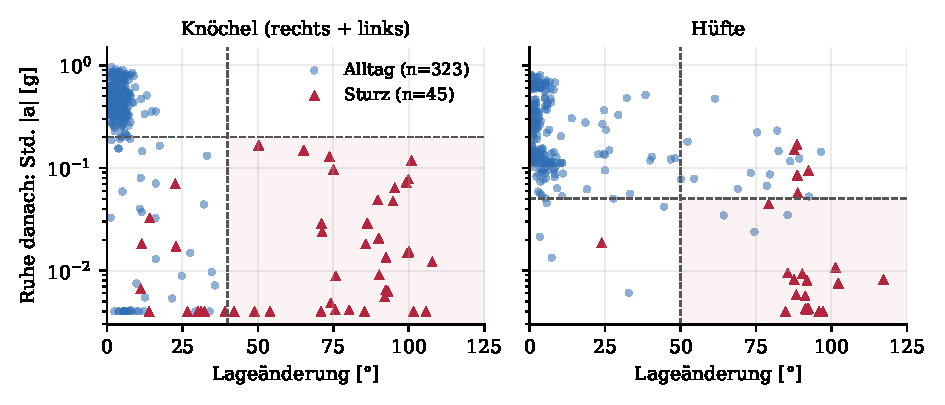
\includegraphics[width=\textwidth]{Bilder/kennwerte_pilot.pdf}
\caption{Lageänderung und Ruhe nach jedem Ereignis (Alltag: jede Spitze
$|a| > 1{,}3$\,g). Rot hinterlegt: Bereich der Regel (zusätzlich
$|a|_{\max} > 1{,}5$\,g). Werte unter $0{,}004$\,g auf $0{,}004$\,g gesetzt.}
\label{fig:kennwerte}
\end{figure}

\section{Eigene Sohlenaufnahmen}
\label{sec:sohle}
Zum Projektende wurden mit dem Prototyp Aufnahmen in beiden Sohlen
erstellt (eine Person, 26 Dateien, $19{,}9$\,min, $100$\,Hz,
$\pm 16$\,g, ohne Sättigung): vier Sturzarten sowie Gehen, Joggen,
Treppen, Springen und kräftiges Hinsetzen. Stürze auf die Knie fanden auf
hartem Boden statt, die übrigen auf einer weichen Unterlage. Bereits ohne
Modell zeigt sich: \textbf{Kein Sturz übertrifft die stärkste
Alltagsbewegung.} Rechts erreicht Joggen $6{,}5$\,g, die Stürze
$2{,}3$--$5{,}4$\,g; links Springen $7{,}7$\,g, die Stürze
$3{,}5$--$5{,}7$\,g. Normales Gehen erreicht an der Sohle über $4$\,g und
damit mehr, als die bisherige Partner-Sohle ($\pm 2$\,g je Achse,
höchstens $3{,}5$\,g als Betrag) messen kann. Die Aufnahmen bestätigen
damit an der Zielposition, dass nur die zeitliche Form trennt; ihre
Auswertung mit dem Modell steht noch aus.

\section{Kommerzielles Modell}
\label{sec:kommerz}
\begin{table}[H]
\centering\small
\caption{Kommerzielles Modell (ohne Smart-Insole und MobiAct) gegenüber
B2r auf identischen Falten. Smart-Insole und Pilotdaten sind für beide
extern.}
\label{tab:kommerz}
\begin{tabularx}{\textwidth}{Y c c c c c}
\toprule
\textbf{Modell} & \textbf{Se} & \textbf{Se gedreht} & \textbf{FP/h IMB} & \textbf{FP/h SI} & \textbf{Pilot Knöchel Se} \\
\midrule
B2r (Bericht)        & \offen{} & \offen{} & \offen{} & \offen{} & \offen{} \\
Kommerziell          & \offen{} & \offen{} & \offen{} & \offen{} & \offen{} \\
\bottomrule
\end{tabularx}
\end{table}
\offen{Einordnung nach dem Lauf von Notebook~05, Teil~E: gesicherter
Unterschied ja/nein, in welche Richtung.}

\section{Übersicht der geprüften Behauptungen}
\begin{table}[H]
\centering\footnotesize
\setlength{\tabcolsep}{3pt}
\caption{Geprüfte Behauptungen und Ergebnis.}
\label{tab:hypothesen}
\begin{tabularx}{\textwidth}{>{\raggedright\arraybackslash}p{5.6cm} c Y}
\toprule
\textbf{Behauptung} & \textbf{Ergebnis} & \textbf{Beleg} \\
\midrule
Fine-Tuning schließt die Domänenlücke & \ja & UMAFall Taille $46 \rightarrow 94\,\%$, FallAllD $11 \rightarrow 76\,\%$; Spezifität bleibt \\
Sturzdaten vom Bein sind für das Fußmodell nötig & \ja & Schienbein $+61{,}5$\,pp (B1 vs.\ K, 5/5 Falten) \\
Die Achsenlage erklärt den Links-rechts-Unterschied & \ja & Spiegelung links: $5 \rightarrow 54\,\%$, rechts: $47 \rightarrow 4\,\%$ \\
Ein Gyroskop verbessert die Erkennung deutlich & \teils & RF: $62\,\%$ Gyro-Wichtigkeit; CNN an der Hüfte nur $+1{,}3$\,pp (Deckeneffekt) \\
Höhere Abtastrate sichert den Transfer & \nein & FallAllD ($238$\,Hz) $11{,}3\,\%$, KFall ($100$\,Hz) $99{,}5\,\%$ \\
Der Messbereich $\pm 8$\,g erklärt den FallAllD-Einbruch & \nein & Clipping auf $\pm 8$\,g: unverändert $99{,}0\,\%$ \\
Die Position bestimmt die Leistung & \nein & Seite (Achsenlage) wiegt schwerer: Spiegeltest $5 \rightarrow 54\,\%$ \\
Progressives Fine-Tuning hilft & \teils & $+23{,}8$\,pp bei wenig Zieldaten; bei vielen kein Unterschied (L0 vs.\ B2) \\
Hard Negatives senken Fehlalarme sinnvoll & \nein & $+1{,}8$\,pp Sp gegen $-6{,}3$\,pp Se \\
Voting senkt Fehlalarme & \teils & 3 von 5: $-70\,\%$ FP, aber $-40\,\%$ erkannte Stürze (UMAFall-Knöchel) \\
Ältere erzeugen mehr Fehlalarme & \teils & Handgelenk: v.\,a.\ Klatschen, Türöffnen; Sohle: ja ($127$ vs.\ $69$/h) \\
Fußdaten ohne Stürze kosten Sensitivität & \nein & augmentiert: Se $-0{,}2$\,pp (n.\,s.), FP $-91$ bis $-96\,\%$; ohne Augm.\ Sp $-8{,}6$\,pp \\
Augmentierung kostet Sensitivität & \nein & Se $+0{,}8$\,pp (n.\,s.), gedreht $+17{,}9$\,pp, FP an Smart-Insole geringer \\
Das Basismodell scheitert an der eigenen Hüfte wegen der Hardware & \nein & Achsen wie SisFall: $2 \rightarrow 15$ von 22 \\
Spitzenwerte trennen Stürze am Fuß & \nein & Knöchel: Alltag bis $10{,}7$\,g; Sohle: Stürze $\leq 5{,}7$\,g, Joggen/Springen bis $7{,}7$\,g \\
Smart-Insole im Training senkt Fehlalarme weiter & \teils & $28 \rightarrow 11$/h, aber Se $-2{,}0$\,pp (gesichert) \\
Breiteres Vortraining verbessert das Fußmodell & \offen{} & Notebook 05, Teil E \\
\bottomrule
\end{tabularx}
\end{table}

\section{Einschränkungen}
Eigene Sohlenaufnahmen mit Stürzen liegen erst seit Projektende vor
und sind mit dem Modell noch nicht ausgewertet; das Firmwaremodell ist
an der Sohle daher nicht validiert, sondern vom Knöchel übertragen. Die
Pilotdaten stammen von einer Person und enthalten nur Minuten Alltag.
Alle Stürze sind simuliert, von überwiegend jungen Personen. Die
Aufprallbeschriftung von CAPPIMU ist eine Näherung.

%==================================================================
\chapter{Zusammenfassung und Ausblick}
\label{ch:fazit}
%==================================================================
Eine Sturzerkennung in der Einlegesohle ist mit einer 6-Achsen-IMU und
einem kleinen 1D-CNN auf dem ESP32-C6 umsetzbar; das Modell benötigt
rund $77$\,KB und rechnet alle $200$\,ms. Die wesentlichen Erkenntnisse:

\begin{enumerate}\setlength\itemsep{1pt}
\item \textbf{Am Fuß sind Fehlalarme das Kernproblem}, nicht die
      Sensitivität. Ein auf Beinstürze trainiertes Modell ohne
      Sohlendaten erzeugt an der Sohle $268$--$400$ Fehlalarme je
      Stunde, das Rumpfmodell $65$--$101$, bei Älteren $127$.
\item \textbf{Die richtigen Daten wirken stärker als jede andere
      Maßnahme.} Sturzdaten vom Bein heben die Sensitivität um $61$\,pp,
      Sohlendaten ohne Stürze senken die Fehlalarme um $91$--$96\,\%$,
      ohne Sensitivität zu kosten (augmentiert). Umgewichtung (Hard
      Negatives) und Voting allein reichen nicht. Ein Grenzwert auf die
      Spitze kann an der Sohle grundsätzlich nicht trennen.
\item \textbf{Die Achsenlage des Sensors ist eine eigene, bislang
      übersehene Fehlerquelle.} Sie erklärt den Seitenunterschied
      vollständig und den Einbruch an der eigenen Hüfte weitgehend.
      Die Einbaulage gehört zur Modellspezifikation und wird in der
      Firmware ausgeglichen; eine Rotationsaugmentierung macht das
      Modell zusätzlich robust.
\item \textbf{Auf der eigenen Hardware} erkennt B2r nach Ausrichtung über
      die Schwerkraft alle 67 Stürze einer Person an Hüfte und Knöcheln.
\end{enumerate}

\textbf{Ausblick.} (1) Die vorhandenen Aufnahmen in beiden Sohlen mit
dem Modell auswerten und um mehrere Personen und Stürze auf hartem Boden
ergänzen, um das Modell an der Zielposition zu validieren. (2) Zweite Stufe mit
Lageänderung und Liegephase zur Bestätigung eines Alarms und
Langliegeerkennung. (3) Parameter der Alarmlogik ($N$, $M$, Schwelle)
auf Sohlendaten festlegen. (4) Energiebedarf im Dauerbetrieb messen.
(5) Für NEARBY (vormals Clever-Sole) das kommerzielle Modell nach
Prüfung der Lizenzen übergeben.

\bibliography{references}

\end{document}
